\chapter{Methodik}

Dieses Kapitel beschreibt die methodische Umsetzung des in dieser Arbeit entwickelten Similarity-Hash-Verfahrens zur Videoquellenerkennung mittels MP4-Container-Analyse. Zunächst wird in \cref{sec:design} das Untersuchungsdesign anhand eines Verfahrenssteckbriefs eingeordnet. Anschließend widmet sich \cref{sec:feature} der Extraktion und Repräsentation der strukturellen Merkmale aus der MP4-Baumstruktur, während \cref{sec:aehnlichkeit} die Berechnung der Ähnlichkeitswerte sowie deren Klassifikation beschreibt. Darauf aufbauend erläutert \cref{sec:vorgpipe} das grundlegende und technische Vorgehen sowie die daraus abgeleitete Datenpipeline. Abschließend stellt \cref{sec:kidatensatz} den im Rahmen dieser Arbeit erstellten eigenen Datensatz aus KI-generierten Videos vor, der die etablierten Referenzdatensätze um synthetisch erzeugtes Test- und Trainingsmaterial ergänzt.

\section{Untersuchungsdesign}

% Verfahrensteckbrief me

\begin{table}[H]
    \centering
    \begin{tabular}{>{\raggedright\arraybackslash}p{0.2\linewidth}>{\raggedright\arraybackslash}p{0.75\linewidth}}\toprule\toprule
         \textbf{Verfahren}& Syntaktisches Similarity Hashing\\\hline\hline
         \textbf{Untersuchungsziele}& SCI (Unterscheidung nativer Kameraaufnahmen und KI-generierter Videos) und SNA (Erkennung komprimierter Social-Media-Videos)\\\hline
         \textbf{Feature}& Extrahierte 4CC-Box-Informationen unter Ausschluss der Inhaltsdaten (\(mdat\)) und volatile Metadaten (z. B. Zeitstempel wie \(creationTime\))\\\hline
         \textbf{Symbolische Repräsentation} (T1 bis T5)& TODO: linearisiert die in JSON erfasste hierarchische Baumstruktur in eindimensionale Token-Sequenzen, ohne vertikale Pfade zu extrahieren\\\hline
         \textbf{Feature-Repräsentation}& n-Gramm-Sets (Similarity Digest)\\\hline
         \textbf{Feature-Selektion}& Allowlisting relevanter Container-Boxen und Dubletteneliminierung\\\hline
         \textbf{Klassifikator}& Approximate Matching (Ähnlichkeitsberechnung mittels Jaccard-Index oder asymmetrischem Tversky-Index)\\\hline
         \textbf{Datenbanken}& VISION, EVA-7K und ein eigens erstellter Datensatz zu KI-generierten Videos\\\hline
         \textbf{Test- und Trainingsdaten}& Bildung von Referenz-Hashes (Source Similarity Digests) aus einer kleinen, diversen Teilmenge (z. B. ein Bild pro Aufnahmemodus), Abgleich mit allen restlichen Testdateien\\\hline
         \textbf{Evaluation}&Native Aufnahmen, Social Media, synthetische Inhalte und gemischte Inhalte\\\hline
         \textbf{Metriken}&Receiver Operating Characteristic (ROC) und Area Under Curve (AUC)\\ \bottomrule\bottomrule
    \end{tabular}
    \caption{Verfahrenssteckbrief zum Similartiy Hashing für Mp4-Dateien (Eigene Darstellung)}
    \label{tab:steckbrief-mp4}
\end{table}
\section{Feature-Engineering für MP4-Container}

TODO: Weitere Stichpunkte für alle Unterkapitel sammeln und ausformulieren

\subsection{Feature-Extraktion und Feature-Selektion}

\begin{itemize}
    \item Auslesen der Datei über eigenen Parser (speichereffizient per Memory Mappin)
    \begin{itemize}
        \item Transparenz nicht nur "was" sondern "wie"
    \end{itemize}
    \item Extraktion der Boxen 8-Byte-Header (Größe und 4CC-Bezeichner) 
    \item Inhalt der mdat ignorieren
    \item Volatile Metadaten (z. B. \verb|creationTime|, \verb|modificationTime|, \verb|duration|, Dateigröße) werden ausgeschlossen (Buzzwort: Exklusion)
    \item Definition, welche Boxen als Container definiert sind (Buzzwort: Allowlisting)
    \begin{itemize}
        \item Basis Standard ISO/IEC 14496-12: \textbf{moov, trak, mdia, minf, stbl, udta, meta, edts, dinf, stsd, mvex, moof, traf, mfra} \cite{iso_14496-12_2022}
    \item Codec-Erweiterungen ISO/IEC 14496-14 und -15 : \textbf{mp4a, avc1, hev1} \cite{iso_14496-14_2020}\cite{iso_14496-15_2024}
    \item Legacy aus Apple-Quick-Time-Zeiten: \textbf{gmhd, clip, matt, wave}\cite{apple_quicktime_2001}
    \item Siehe \cref{tab:mp4allowlisting}
    \end{itemize}
    \item Erlaubte Container werden rekursiv nach Boxen durchsucht
    \item Berücksichtigung von Apple-Quick-Time-Boxen (Buzzwort: Legacy)
    \item Beachtung von Offset-Sprüngen siehe \cref{tab:mp4ausnahmeboxen} (Buzzwort: FullBox)
    \item Boxen außerhalb der Allowlist werden als Bätter/Leafs behandelt
    \item Extraktion im JSON-Format
\end{itemize}

\begin{table}[h]
    \centering
\caption{Valide MP4-Container gem. ISO/IEC 14496-12, -14, -15 und Apple Quick Time Legacy}
\label{tab:mp4allowlisting}
    \begin{tabular}{|l|p{2.5cm}|p{5.5cm}|p{5.5cm}|}\hline
         \textbf{Typ (4CC)}&  \textbf{Bezeichnung}&\textbf{Kurzbeschreibung}&\textbf{Besonderheiten}
\\\hline
         moov&  Movie Box&Haupt-Container für alle Metadaten des Videos& keine\\\hline
         trak&  Track Box&Einzelne Medienspur (Video, Audio oder Daten).& keine\\\hline
         mdia&  Media Box&Informationen über die Medienformate innerhalb eines Tracks& keine\\\hline
         minf&  Media Information&Container für Handler-spezifische Informationen& keine\\\hline
         stbl&  Sample Table&Zeitstempel, Größen und Offsets& keine\\\hline
         udta&  User Data&Benutzerdefinierte Metadaten (oft Hersteller-Tags)& keine\\\hline
         meta&  Metadata&Moderne Metadaten-Strukturen (z. B. C2PA oder EXIF).& Zweideutige Struktur, die in der ISO-Norm und in Apple-Legacy unterschiedlich spezifiziert sind\\\hline
         edts&  Edit Box&Definiert Abspiel-Modifikationen (z. B. Audio-Offsets).& keine\\\hline
         dinf&  Data Information&Verweist auf den Ort der eigentlichen Mediendaten& keine\\\hline
 stsd& Sample Description&Container für Codec-spezifische Konfigurationsdetails& Definierte sog. FullBox und besitzt erweiterte Header-Daten\\\hline
 avc1& H.264 Entry&Parameter des H.264 Videocodecs&Beinhaltet massive binäre Parameter, welche die Baumstruktur unterbrechen und gesondert behandelt werden müssen\\\hline
 hev1& HEVC Entry&Parameter des H.265 (HEVC) Videocodecs&Beinhaltet massive binäre Parameter, welche die Baumstruktur unterbrechen und gesondert behandelt werden müssen\\\hline
 mp4a& Audio Entry&Container für Audio-Codec-Einstellungen (z. B. AAC).&Beinhaltet massive binäre Parameter, welche die Baumstruktur unterbrechen und gesondert behandelt werden müssen\\\hline
 wave& QuickTime Audio&Alte Audio-Eigenschaften (Legacy)& keine\\\hline
 mvex& Movie Extends&Kennzeichnet die Nutzung von Fragmented MP4 (Streaming).& keine\\\hline
 moof& Movie Fragment&Metadaten für einzelnes Video-Fragment& keine\\\hline
 traf& Track Fragment&Informationen innerhalb eines Movie Fragments& keine\\\hline
 mfra& Movie Fragment Random Access&Index für den schnellen Zugriff auf Fragmente& keine\\\hline
 gmhd& Generic Media Header&QuickTime-Container für allgemeine Medieninfos (Legacy)& keine\\\hline
 clip& Clipping Box&Bestimmt den sichtbaren Bereich des Videos (Legacy)& keine\\\hline
 matt& Track Matte Box&Definiert Masken für die Videospur (Legacy).& keine\\ \hline
    \end{tabular}
\end{table}
\begin{table}[h]
    \centering
\caption{Ausnahmeregelungen und Offset-Korrekturen beim Parsing}
\label{tab:mp4ausnahmeboxen}
    \begin{tabular}{|l|p{4.5cm}|p{6.5cm}|}\hline
         \textbf{Typ (4CC)} & \textbf{Strukturelle Abweichung im Binärstrom} & \textbf{Implementierte Lösungslogik (Offset-Korrektur)} \\\hline
         meta & Spezifikationskonflikt zwischen Apple-Legacy (Standard-Container) und neuer ISO-Norm (FullBox mit Versions- und Flag-Bytes) & Vorschau der ersten 4 Bytes und bei Detektion von Null-Bytes (\texttt{0x00000000}) erfolgt ein Offset-Sprung von +4 Bytes, andernfalls +0 Bytes \\\hline
         stsd & Container ist als FullBox deklariert und erzwingt im Anschluss einen zusätzlichen 32-Bit-Zähler & Start-Offset für den rekursiven Abstieg in die Unterboxen wird fix um +8 Bytes verschoben \\\hline
         avc1, hev1 & Visuelle Sample Entries und weisen direkt nach dem Header zwingend 78 Bytes an binären Bildparametern auf, bevor Unterboxen beginnen & Überspringen der binären Videodaten durch eine Offset-Verschiebung von +78 Bytes\\\hline
         mp4a & Auditiver Sample Entry und weist nach dem Standard-Header zwingend 28 Bytes an binären Audioparametern auf & Überspringen der binären Audiodaten durch eine Offset-Verschiebung von +28 Bytes\\\hline
    \end{tabular}
\end{table}

%%%

\subsection{Feature-Repräsentation}

\begin{itemize}
    \item Hierarchische MP4-Baum wird in eine eindimensionale Sequenz überführt
    \item \textbf{n-Gramm-Bildung:} Die Sequenz wird mittels eines Sliding-Window-Verfahrens in 2-Gramme überführt 
    \item Fenster ist 8 Zeichen lang (erfasst exakt 2 Token) und verschiebt sich um 4 Zeichen (1 Token) weiter 
    \item Lokale Nachbarschaft unmittelbar benachbarter Boxen bleibt erhalten
    \item   2-Gramme werden zu unveränderlichen Tupeln zusammengefasst 
    \item Durch Überführung in mathematische Mengen (Python-Sets) werden Dubletten eliminiert.
    \item Worthäufigkeiten werden (im Gegensatz zum Bag-of-Words-Modell) ignoriert 
    \item Ergebnis ist eine bereinigte, alphabetisch sortierte Signatur (Buzzwort: Similarity Digest)
\end{itemize}

\section{Ähnlichkeitsanalyse und Klassifikation}

\label{sec:aehnlichkeit}
\section{Vorgehen und Datenpipeline}

TODO: 5 schritte (Best Practice) struktur-extraktion, feature-exktraktion, feature-selektion, feature-repräsentation und klassifikation \cite[Fig. 4]{yang_comprehensive_2025}

\subsection{Vorgehen}

TODO: Stichpunkte ausformulieren

% Grafik des Vorgehens

\begin{figure}[H]
    \centering
    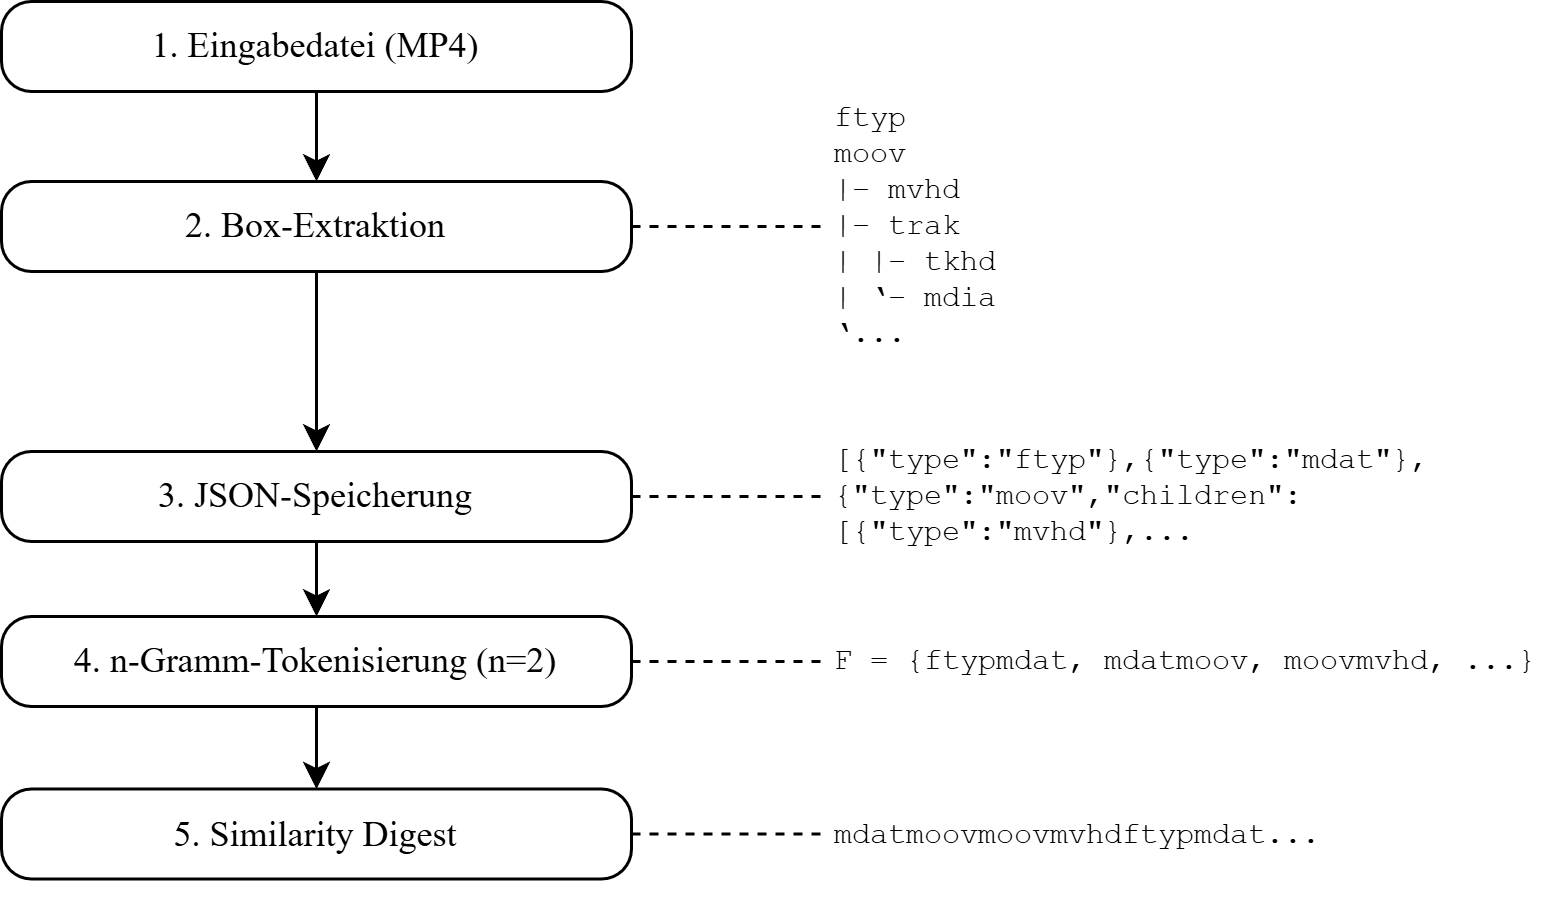
\includegraphics[width=1\linewidth]{grafiken/vorgehen-mp4.drawio.png}
    \caption{TODO: vorgehen-mp4.drawio.png}
    \label{fig:vorgehen}
\end{figure}

% Stichpunkte Vorgehen

\begin{enumerate}
    \item Mp4 Dateien parsen
    \item Box-Informationen extrahieren
    \item Box-Struktur im JSON-Format abspeichern
    \item Box-Struktur linearisieren und als 2-Gramme tokenisieren
    \item 2-Gramme als Similarity Digest abspeichern und die mit 8-Zeichen-Fenster auslesbar sind
\end{enumerate}

%%%

\newpage
\subsection{Datenpipeline}

GitHub: \url{https://github.com/lmechelk/mp4-similarity-hash/}\\

TODO: Stichpunkte ausformulieren

% BPMN der Pipeline

\begin{figure}[H]
    \centering
    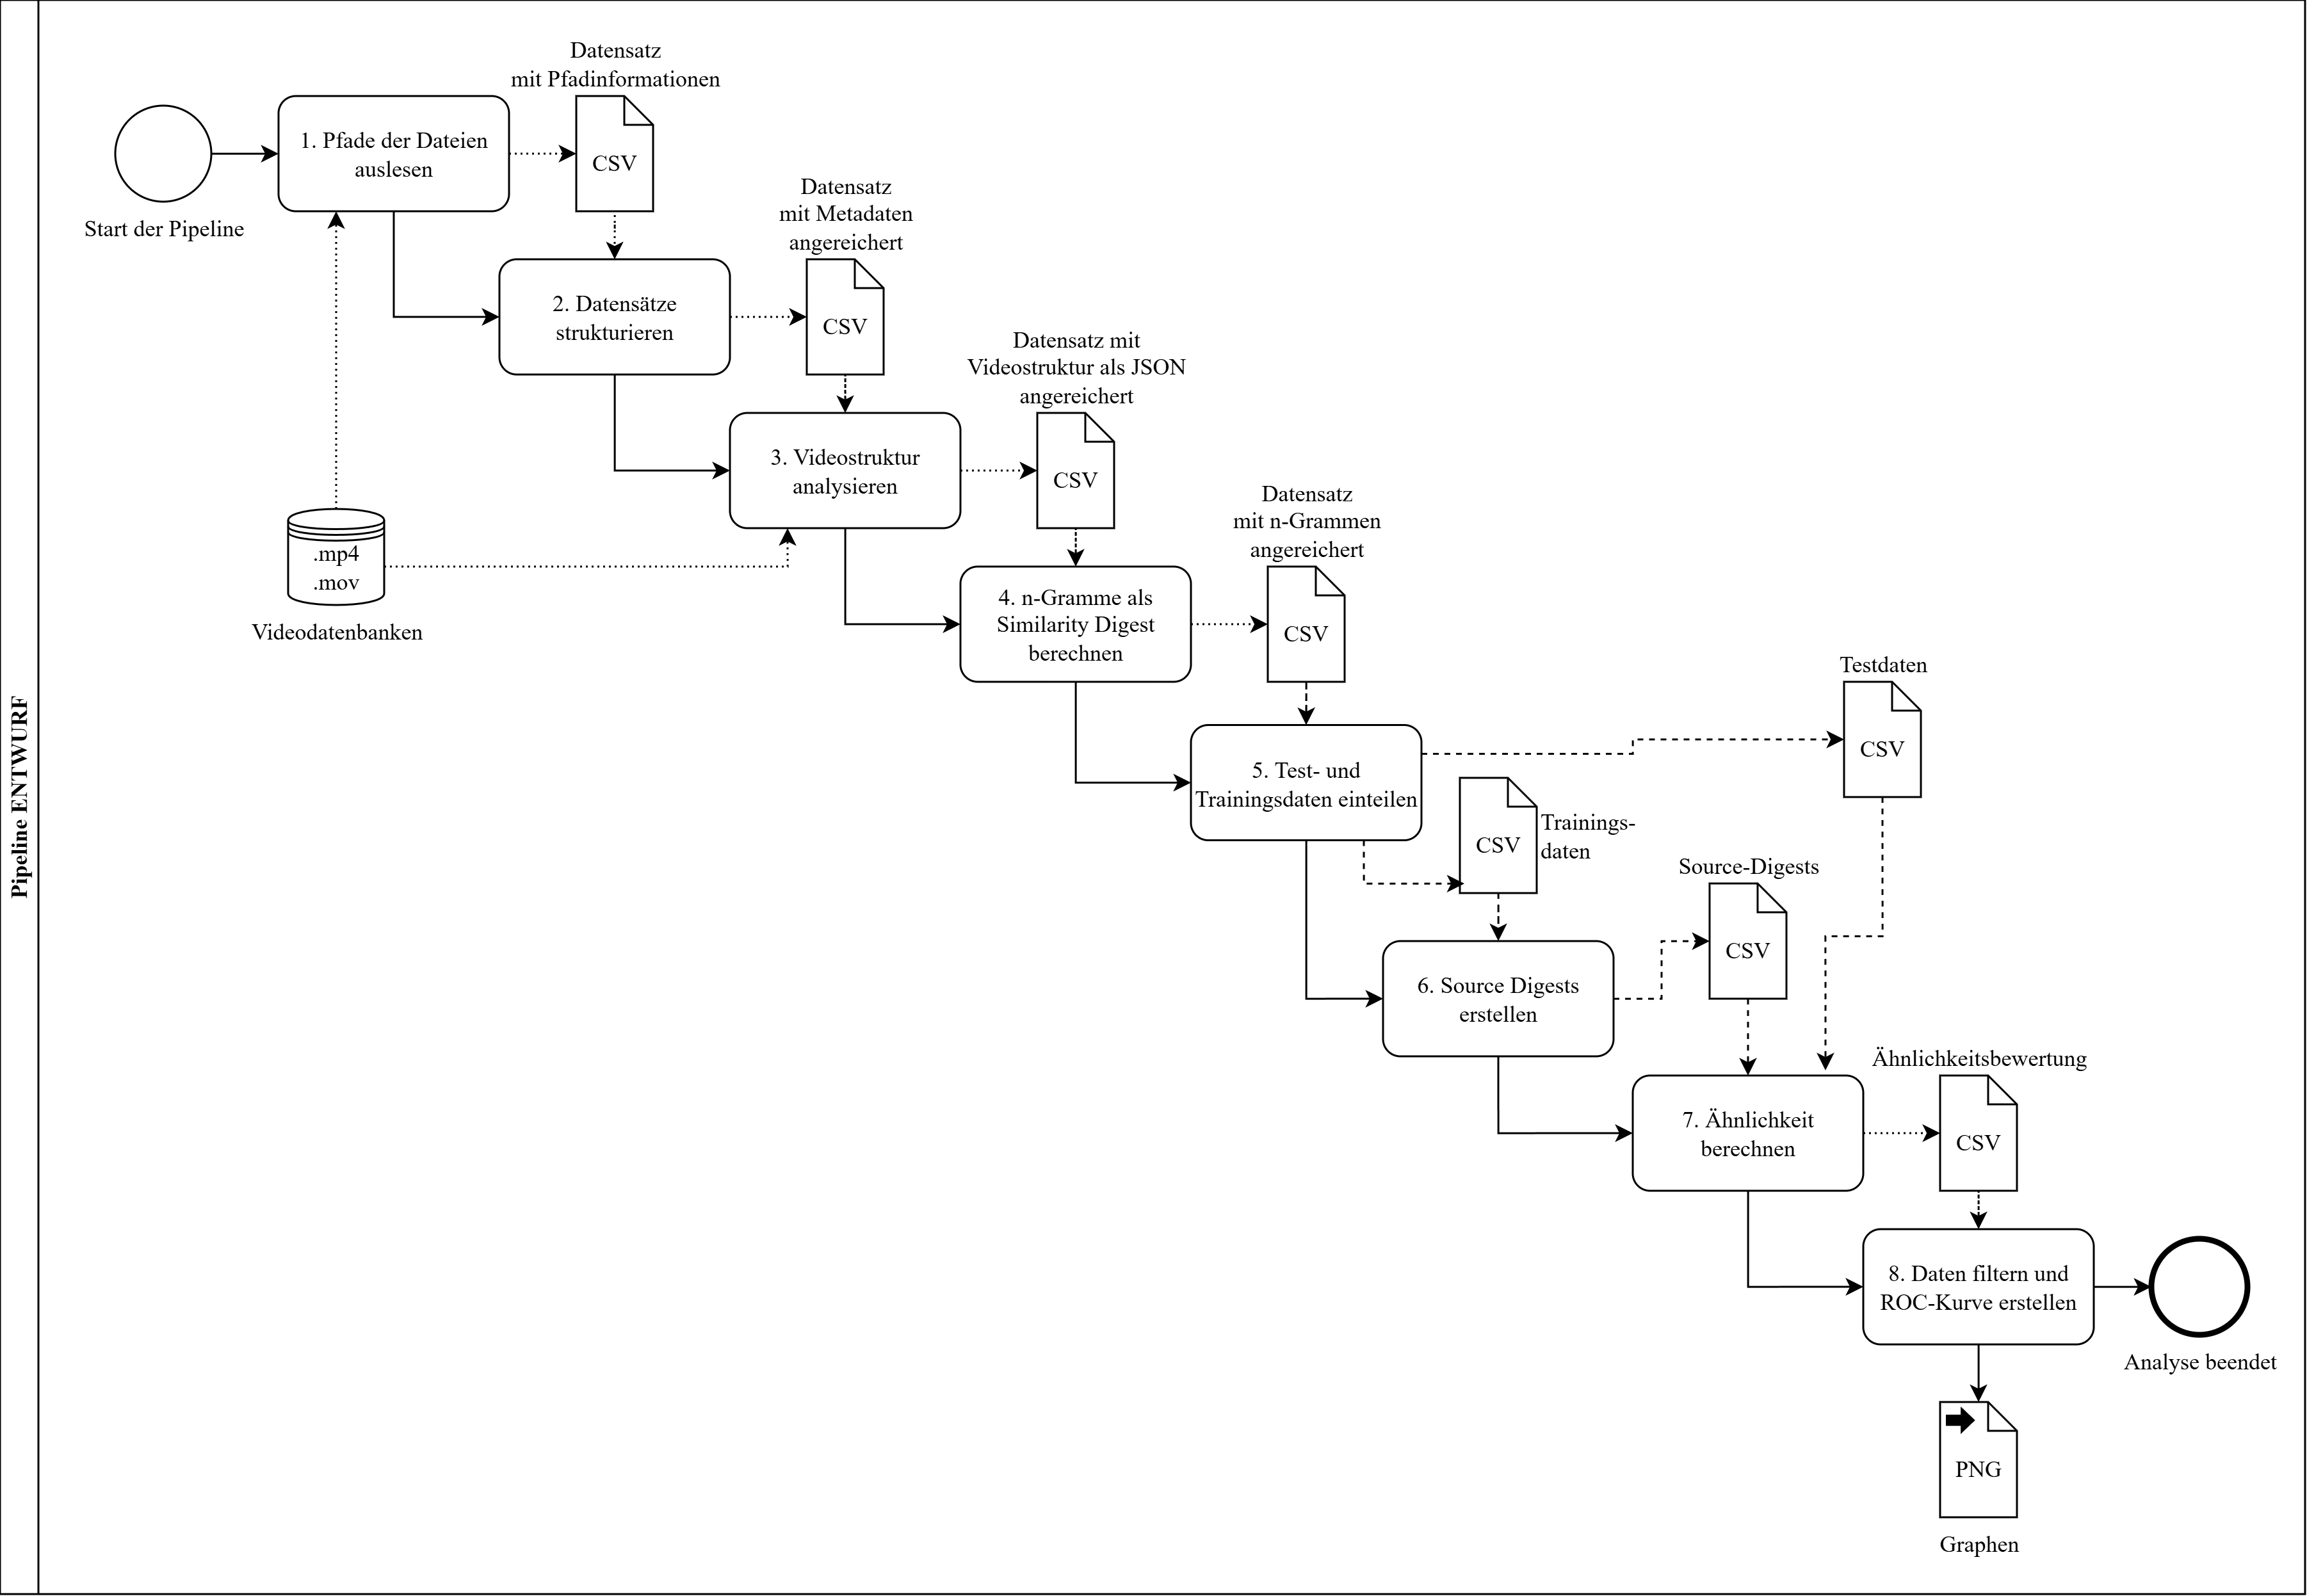
\includegraphics[width=1\linewidth]{grafiken/pipeline.drawio.png}
    \caption{TODO: pipeline.drawio.png}
    \label{fig:pipeline}
\end{figure}

% Stichpunkte Pipeline

\begin{enumerate}
    \setcounter{enumi}{-1}
    \item \textbf{Videodatenbanken bereitstellen}
    \begin{itemize}
        \item EVA-7k (5.684 Dateien)
        \item VISION (nur Videos, 1918 Dateien)
        \item eigener KI-Datensatz
    \end{itemize}
    
    \item \textbf{Pfad jeder einzelnen Videodatei auslesen}
    \begin{itemize}
        \item PATH (Dateipfad z.\,B. \url{C:/Testdaten/EVA/D01_flat_yt.mp4})
    \end{itemize}
    
    \item \textbf{Datensätze strukturieren}
    \begin{itemize}
        \item DB\_NAME (Name der Datenbank z.\,B. Vision, Eva, Selfmade)
        \item ID (Eindeutige Kennung des Geräts (\textit{Device} bei Eva/Vision) oder der AI z.\,B. D01, AI01)
        \item BRAND (Hersteller des Smartphones oder der KI z.\,B. Samsung, Grok)
        \item MODEL (Genaue Version des Smartphones oder der KI z.\,B. GalaxyS3Mini, Imagine\_0.9)
        \item MEDIA\_TYPE (Dateiendung bzw. Containerformat z.\,B. MP4, MOV)
        \item CONTENT\_SOURCE (Originäre Quelle der Videodatei, um zwischen Kameras, vollständig KI-generierten Videos mittels Text-to-Video oder Videos, die auf Bild-Vorlagen basieren (Image-to-Video), zu unterscheiden z.\,B. DIGITAL\_CAMERA, AI\_GENERATION, MIXED)
        \item CONTENT\_TYPE (Kontext der Aufnahme z.\,B. flat, indoor, outdoor, deepfake, synthetic)
        \item PROCESSING (Primäre Verarbeitung des Videos z.\,B. native, youtube, whatsapp, ai)
        \item TAMPERING (Nachträgliche Veränderung des Videos (nur Eva-DB) z.\,B. None, Avidemux)
    \end{itemize}
    
    \item \textbf{Videostruktur analysieren}
    \begin{itemize}
        \item STRUCTURE\_PRETTY (Gut lesbarer String der MP4-Struktur (nur nice to have bzw. zum Debugging) z.\,B. \texttt{moov(mvhd,trak(tkhd))})
        \item STRUCTURE\_JSON (Exakte Baumstruktur als JSON-String, der zur N-Gram-Generierung genutzt wird z.\,B. \verb|[{"type":"moov","children":[{"type":"mvhd"}]}]|)
    \end{itemize}
    
    \item \textbf{$n$-Gramme als Similarity Digest berechnen}
    \begin{itemize}
        \item NGRAM\_2 (Kompakter Similarity Digest (String), der die Signatur des Videos auf Basis von 2-Grammen (alphabetisch, duplikatbereinigt) repräsentiert; jeweils 8 lückenlose Zeichen entsprechen einem 2-Gramm-Feature z.\,B. moovmvhdtrakmvhdtraktkhd)
    \end{itemize}
    
    \item \textbf{Datensätze in Test- und Trainingsdaten einteilen}
    \begin{itemize}
        \item EVA-7k: immer die erste Datei jedes Subsets (avidemux, exiftool, \dots) aus jeder Social-Media-Kategorie (Facebook, TikTok, YouTube, \dots)
        \item VISION: immer die erste Datei jedes Content- (flat, indoor, \dots) und Processing-Types (Original, Facebook, \dots) aus jedem Device
        \item eigener KI-Datensatz: immer die erste Datei jedes KI-Modells
    \end{itemize}
    
    \item \textbf{Source-Digest erstellen}
    \begin{itemize}
        \item Digest für jede Kategorie anhand der Testdaten generieren, z.\,B. gruppiert nach Brand, Device, Social-Media, KI, KI-Modell
        \item SOURCE\_DIGEST (aggregierter Similarity Digest)
    \end{itemize}
    
    \item \textbf{Ähnlichkeit berechnen}
    \begin{itemize}
        \item GROUND\_TRUTH\_SOURCE\_DIGEST: Bezeichner für die Ground Truth, anhand der die Testdaten erstellt wurden
        \item GROUND\_TRUTH\_MP4: Bezeichner für die Ground Truth der einzelnen Test-MP4
        \item SIMILARITY: Wert von 0 bis 1 gem. Tversky-Berechnung (kein Penalty bei fehlenden Boxen in Testdatei, Penalty bei zusätzlichen Boxen in Testdatei)
    \end{itemize}
    
    \item \textbf{Daten filtern und auswerten}
    \begin{itemize}
        \item ROC und AUC berechnen
        \item Graphen erstellen
    \end{itemize}
\end{enumerate}

\begin{table}[htbp]
    \centering
    \resizebox{\textwidth}{!}{%
    \begin{tabular}{lllllllllll}
        \toprule
        \textbf{DB\_NAME} & \textbf{ID} & \textbf{BRAND} & \textbf{MODEL} & \textbf{MEDIA\_TYPE} & \textbf{CONTENT\_SOURCE} & \textbf{CONTENT\_TYPE} & \textbf{PROCESSING} & \textbf{TAMPERING} & \textbf{STRUCTURE\_PRETTY} & \textbf{NGRAM\_2 (Auszug)} \\
        \midrule
        VISION & D15 & Apple & iPhone 6 & MOV & DIGITAL\_CAMERA & FLAT & NATIVE & NONE & \texttt{moov(mvhd,trak(tkhd))} & \texttt{moovmvhdtraktkhd} \\
        EVA-7K & D01 & Samsung & GalaxyS3Mini & MP4 & DIGITAL\_CAMERA & INDOOR & YOUTUBE & AVIDEMUX & \texttt{ftypmoov(mvhd)} & \texttt{ftypmoovmoovmvhd} \\
        SELFMADE & AI01 & Grok & Imagine\_0.9 & MP4 & AI\_GENERATION & SYNTHETIC & AI & NONE & \texttt{ftypuuidmoov(mvhd)} & \texttt{ftypuuiduuidmoov} \\
        \bottomrule
    \end{tabular}%
    }
    \caption{TODO: Beispieldatensätze}
    \label{tab:testdaten_auszug}
\end{table}

TODO: Tabelle mit Auszug der echten Datensätze
% Siehe Anhang Test mit input testdatensätze.tex
\section{Erstellung des Eigenen KI-Video-Datensatzes}
\label{sec:kidatensatz}

Da die etablierten Referenzdatensätze VISION und EVA-7K vor dem technologischen Durchbruch aktueller generativer KI-Modelle entstanden sind, enthalten sie keine synthetisch erzeugten MP4-Container. Zur Schließung dieser Lücke wurde im Rahmen dieser Arbeit ein eigener, frei verfügbarer Datensatz\footnote{Der Datensatz sowie die zugehörige Dokumentation zur Generierung jedes Videos stehen unter \url{https://bit.ly/4wivVOy} zur Verfügung} aus KI-generierten Videos zusammengestellt, dessen Struktur in \cref{tab:ki-modelle} zusammengefasst ist. Eine feingranulare Übersicht des KI-Datensatzes nach Anbieter, Modell, Content-Typ, Erhebungsmethode und thematischen Prompt-Clustern findet sich ebenfalls in der Anlage in \cref{tab:aidb} .

\begin{table}[htbp]
\centering
\begin{tabular}{llll}
\toprule
\textbf{Modell}  
& \textbf{Anbieter}& \textbf{Plattform}& \textbf{Anzahl Dateien} \\
\midrule
Imagine~0.9  
& xAI& Grok 
& 2 \\
Imagine~1.5  
& xAI& Grok 
& 14 \\
Pika~1.5  
& PikaArt& PikaLabs 
& 4 \\
Pika~2.0  
& PikaArt& PikaLabs 
& 4 \\
Pika~2.2  
& PikaArt& PikaLabs 
& 4 \\
Pika~2.5  
& PikaArt& PikaLabs 
& 11 \\
Sora~2  
& Microsoft& Bing& 10 \\
OmniFlash  
& Google& Flow& 4 \\
Veo~3.1  
& Google& Gemini& 4 \\
KlingAIVideo~2.6  
& Kuaishou& KlingAI 
& 2 \\
KlingAIVideo~3.0  & Kuaishou& KlingAI & 2 \\
\midrule
\multicolumn{2}{l}{\textbf{Gesamt}} & & \textbf{61} \\
\bottomrule
\end{tabular}
\caption{Übersicht der verwendeten KI-Generatoren im eigenen Datensatz}
\label{tab:ki-modelle}
\end{table}

Generative KI-Modelle können bereits jetzt fotorealistische Videos anhand von Text-Prompts oder mittels Bildvorlagen generieren und geben diese überwiegend im MP4-Containerformat aus. Die Videodateien des Datensatzes stammen aus zwei unterschiedlichen Quellen. Ein Teil wurde eigenständig über Text- und Bild-Prompts generiert, während ein weiterer Teil direkt aus den frei verfügbaren Katalogen der jeweiligen Anbieter heruntergeladen wurde, um zusätzliche Diversität hinsichtlich Modellversionen und Erzeugungsparametern abzubilden. Die Erstellung sowie Sammlung der Videodateien erfolgte im Zeitraum vom 20.01. bis zum 20.06.2026.

Bei der Auswahl der Generatoren wurde bewusst auf leicht zugängliche und zum Erhebungszeitpunkt aktuelle Modelle zurückgegriffen. Außerdem lag der Fokus auf eine breite Auswahl von Generatoren, um möglichst viele einzigarte Referenz-Source-Digest zu bilden. Die strukturierte Erhebung von forensischem Testmaterial unterliegt bei kommerziellen Modellen erheblichen Limitationen, da die Anbieter restriktive Inhaltsfilter (Safety Guardrails) implementieren, die grundsätzlich die Verarbeitung semantisch kritischer Prompts systematisch verweigern \cite{openai_safety_2025}. Dies zeigte sich insbesondere bei Modellen von Microsoft und Google, die während der Generierung wiederholt die finale Ausgabe des Videos verweigerten, sobald Themen wie Falschinformationen oder simulierte Drohnenaufnahmen adressiert wurden \cite{google_gemini_2023}.

Ein besonderer Schwerpunkt lag dagegen auf Grok, da dieses Modell nahezu jeden Prompt ohne inhaltliche Einschränkung verarbeitet hat \cite{xai_grok_2025}. Diese tolerante Filterarchitektur erweist sich für die Untersuchung von Desinformation und Deepfakes als essenziell, da entsprechende Prompts bei anderen KI-Systemen regelmäßig abgewiesen werden. Auffällig ist zudem, dass die von Grok erzeugten MP4-Container im Gegensatz zu anderen untersuchten Anbietern keine \(uuid\)-Box und damit kein erkennbares C2PA-Manifest enthalten. Dieser Verzicht auf eine kryptografische Authentizitätskennzeichnung fügt sich in das bisherige Gesamtbild von xAI ein und ist hierdurch ein relevantes Unterscheidungsmerkmal.